\chapter{Dados Reais} \label{cap:dadosreais}
\vspace{-2cm}

Durante o período de maio a julho de 2018 foram feitas aquisições de dados do detector para raios cósmicos, utilizando duas pás cintiladoras de dimensões $14$x$14$x$1$ posicionadas acima do plano superior do detector como sistema de acionamento da aquisição (\emph{trigger}). A primeira pá foi posicionada a $4.5$ cm acima da superfície superior do detector enquanto a segunda pá foi posicionada a $47.5$ cm da mesma superfície.

O sistema de \emph{trigger} foi configurado para realizar a aquisição dos dados das PMTs caso ambas as pás cintiladoras tenham detectado um sinal, fazendo a aquisição dos dados salvos nos \emph{buffers} das NDAQs, salvando as últimas $100$ amostras digitalizadas. Foram selecionados no total $9999$ eventos consecutivos registrados pelo detector para análise deste trabalho.



\section{Metodologia de análise dos dados do experimento}

Os dados do experimento são salvos em arquivos de texto com o valor analógico da saída de cada canal de \emph{front-end} convertido para um valor digital que será referido como \emph{ADC counts} a partir deste ponto. Podemos estimar a quantidade de p.e. total por evento validando o valor em \emph{ADC counts} no pico dos sinais coletados, assim, a estratégia para a análise será estimar o pico do sinal em \emph{ADC counts}, converter este valor para p.e. afim de descobrir o valor de energias por PMT e por evento.

Como no sistema existe uma tensão de \emph{bias} negativa, conhecida como pedestal, precisamos removê-la antes de começar uma análise mais profunda dos dados, centralizando nossas amostras no valor nulo. O pedestal pode ser visto e comparado com uma amostra sem o mesmo na Figura \ref{fig:pedestal}.

\begin{figure}[h!]
	\centering
%	\hspace*{-2cm}
	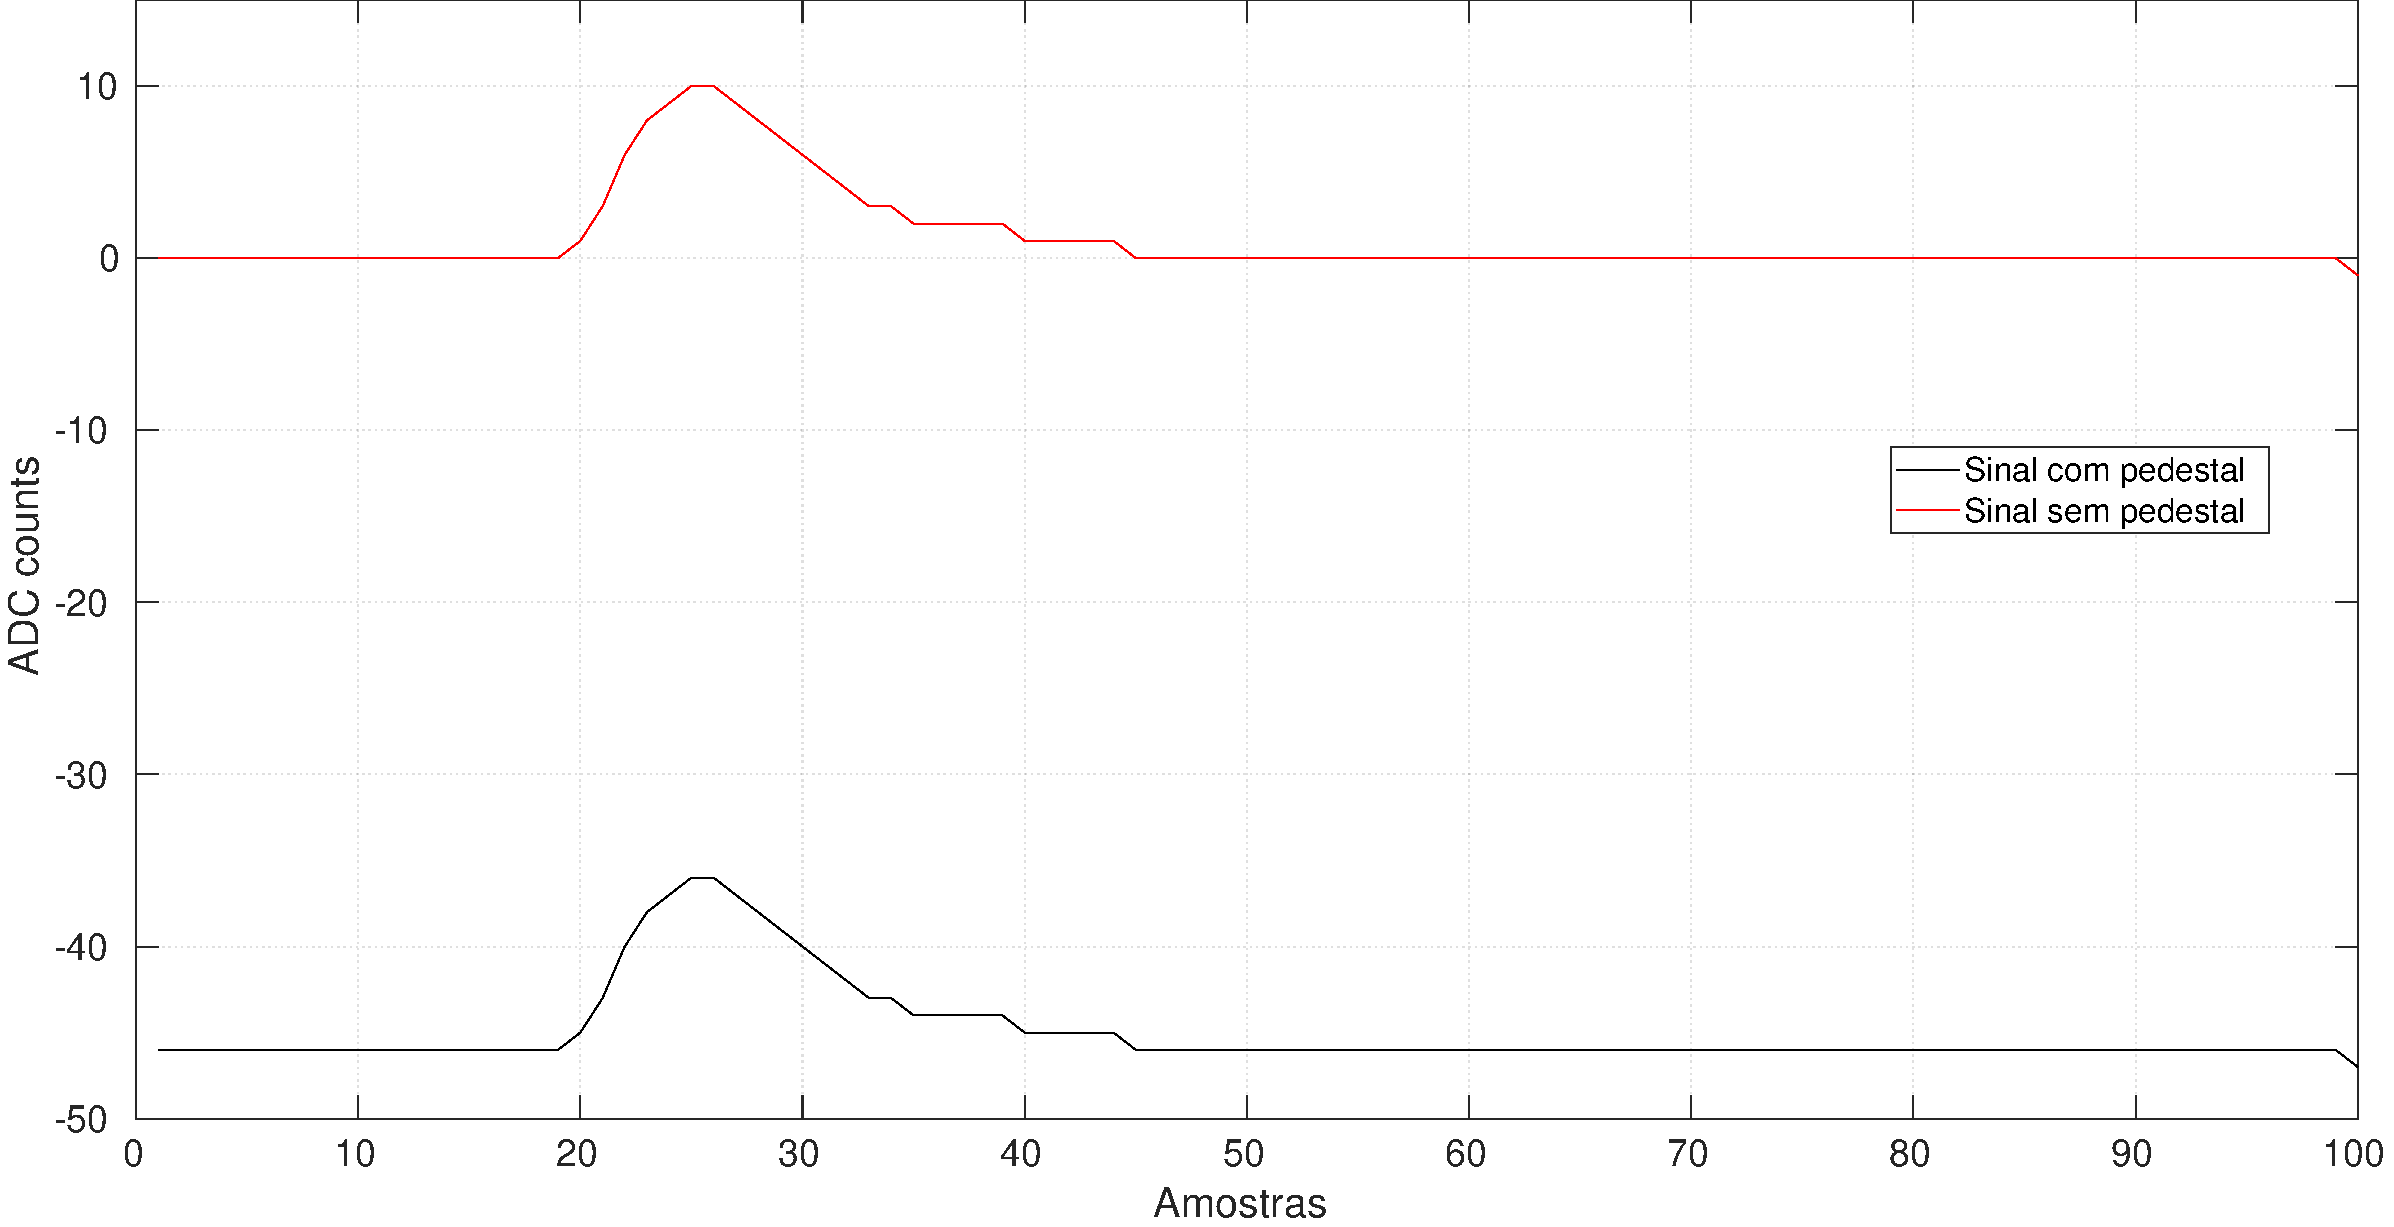
\includegraphics[width=12cm]{textuais/dadosreais/figuras/pedestal.pdf}
	\caption{Sinal com e sem pedestal}
	\label{fig:pedestal}
\end{figure}

Afim de se estimar o número de p.e. coletados por cada PMT, medimos o valor de pico dos sinais gerados pela eletrônica de \emph{front-end}. Devido à saturação das PMTs e da eletrônica de \emph{front-end}, os dados coletados com pico de energia acima do valor de saturação devem ser recuperados de alguma forma. Para isto  foi utilizado um procedimento de \emph{fitting} com uma forma do sinal conhecida através de um processo iterativo, calculando o erro provável de uma área linear pelo teste do $\chi^2$ (qui-quadrado) \cite{vuolo1996fundamentos} e utilizando a forma final com menor erro, estimando assim, a forma do sinal não saturado. Um exemplo de sinal saturado e sua estimação está presente na Figura \ref{fig:sat}.


\begin{figure}[H]
	\centering
%	\hspace*{-2cm}
	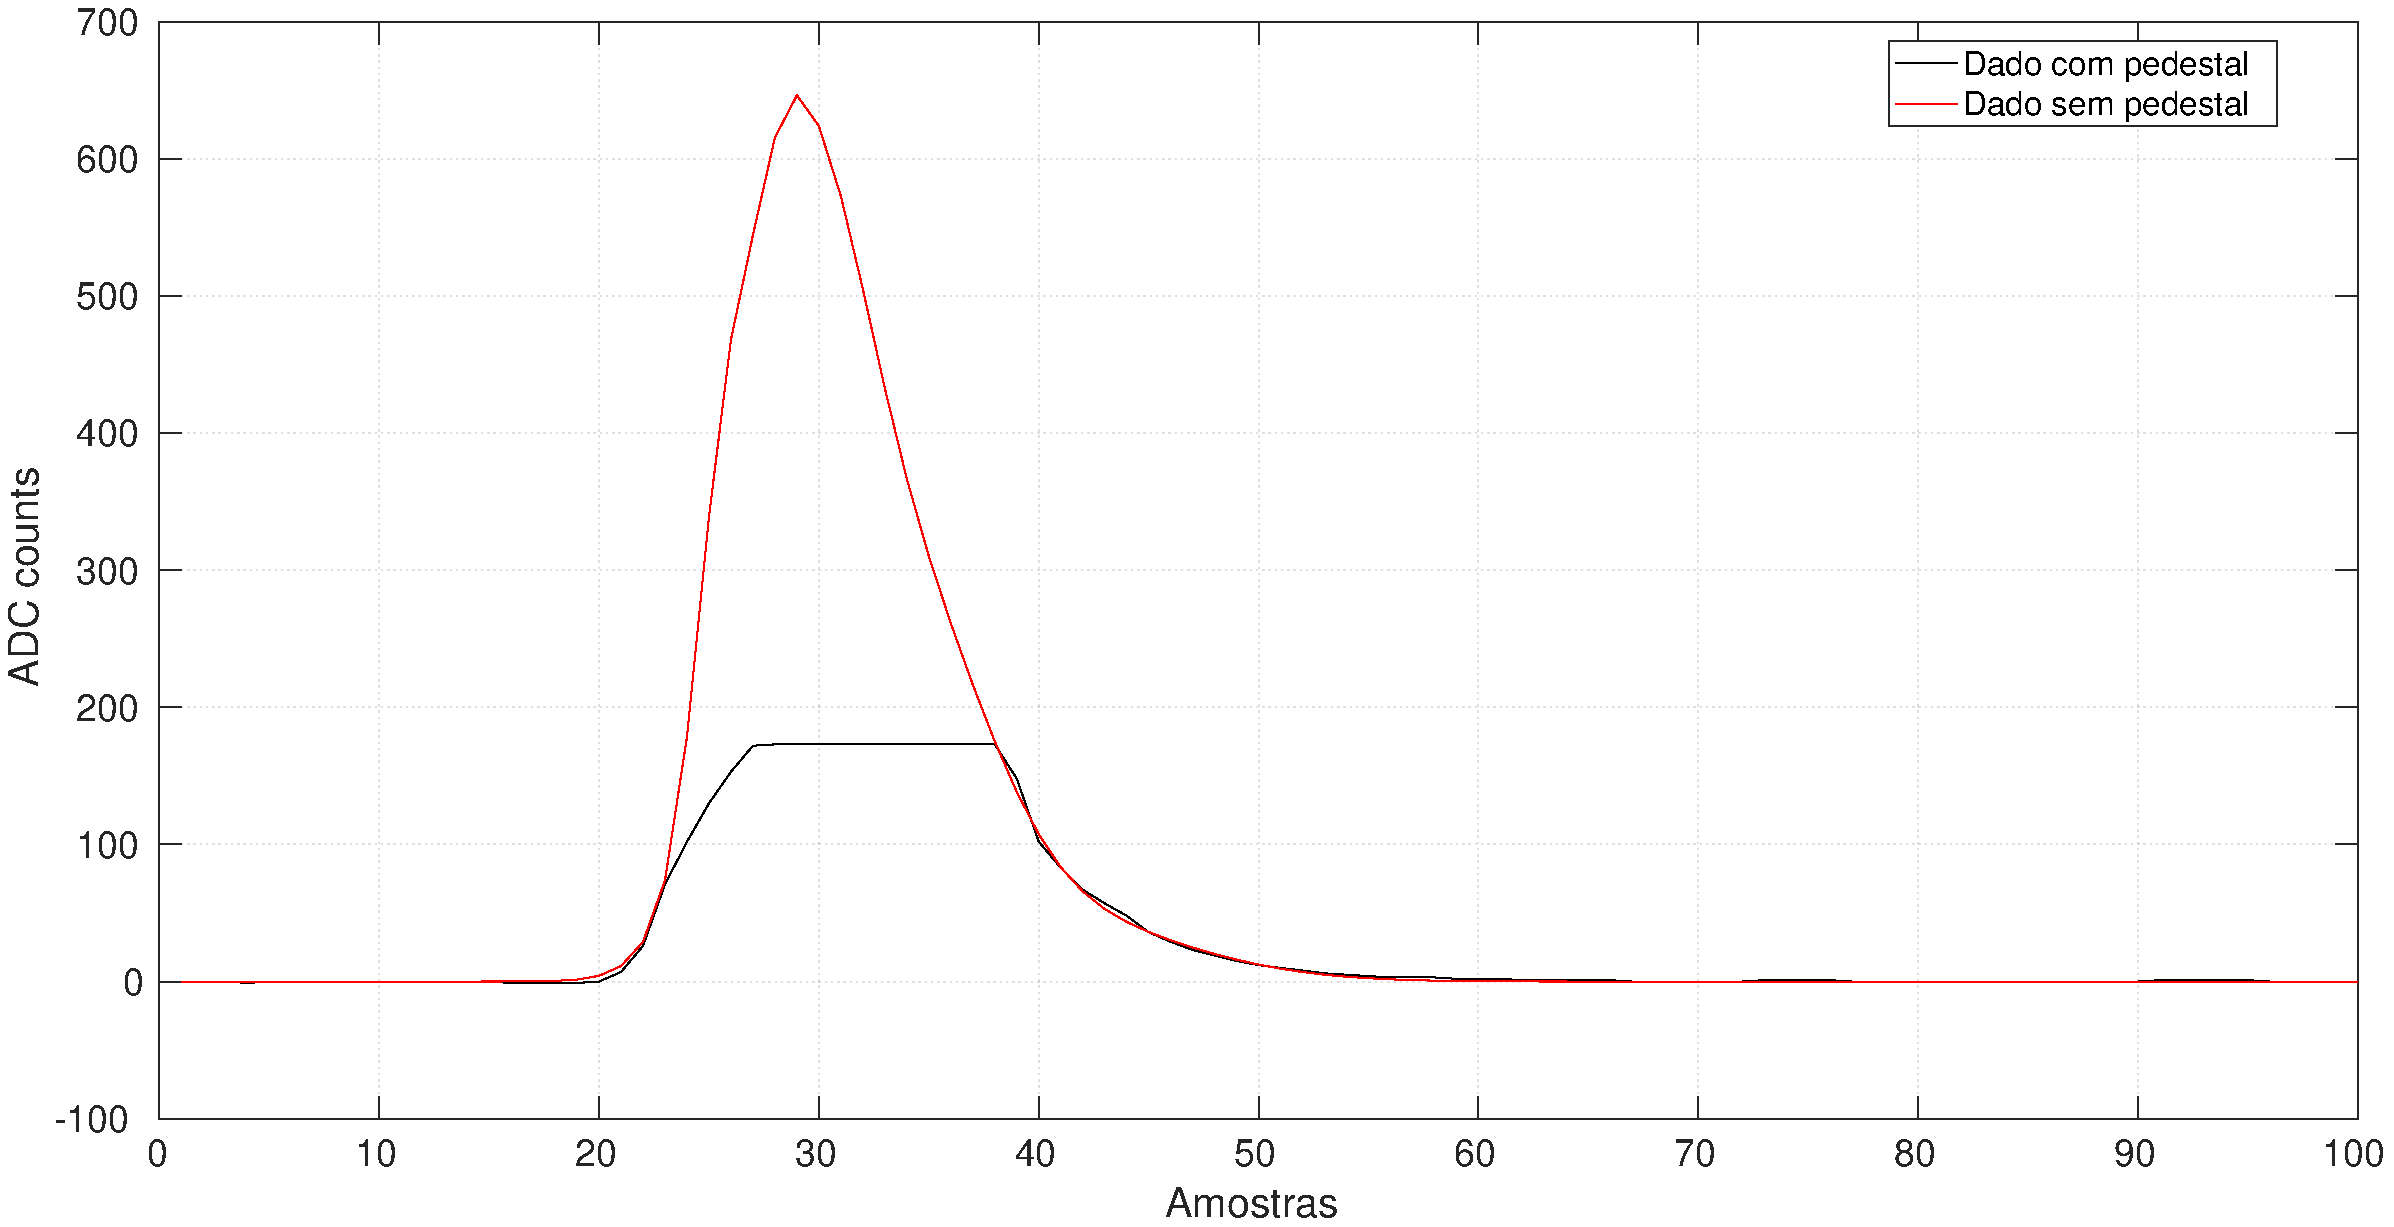
\includegraphics[width=12cm]{textuais/dadosreais/figuras/saturado.pdf}
	\caption{Estimação por regressão}
	\label{fig:sat}
\end{figure}



\section{Debug dos dados reais}


Após o \emph{fit} dos dados, foi encontrado um problema intrínseco ao método, como o \emph{fit} era realizado a partir do ponto de saturação eventos naquele ponto foram, em sua maioria, removidos do sistema como pode ser visto no histograma á esquerda da Figura \ref{fig:peakdist}.

Para resolver este problema precisamos modificar o modo de \emph{fit} a ser realizado. Foi feito então o mesmo método anterior, porém a partir de um ponto em que as PMTs não estão em saturação, mantendo o valor próprio e estimando os valores além do ponto não saturado, resolvendo o erro de estimação e gerando o histograma à direita da Figura \ref{fig:peakdist}.

\begin{figure}[H]
	\centering
%	\hspace*{-2cm}
	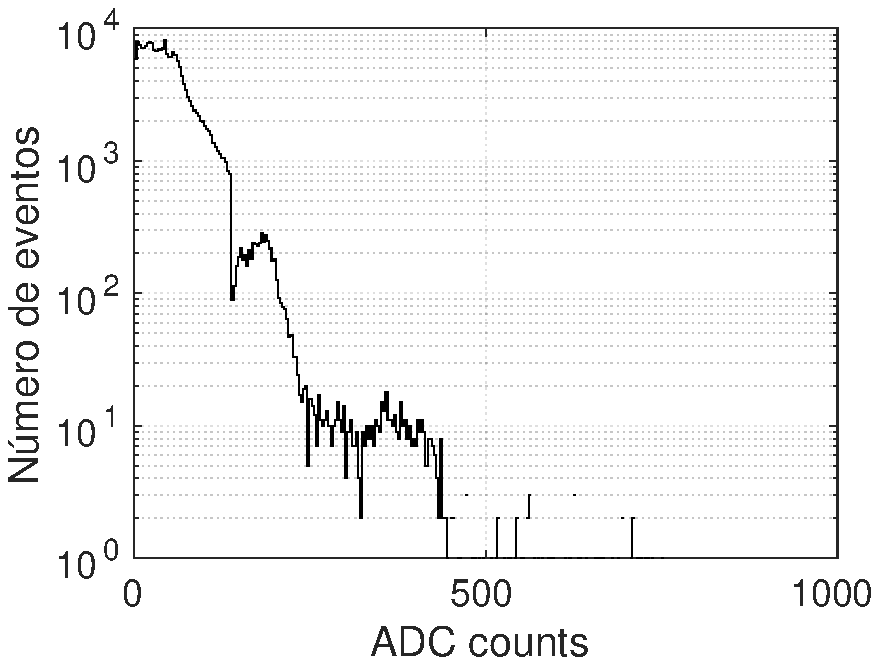
\includegraphics[width=7cm]{textuais/dadosreais/figuras/peakdist_errado.pdf}
	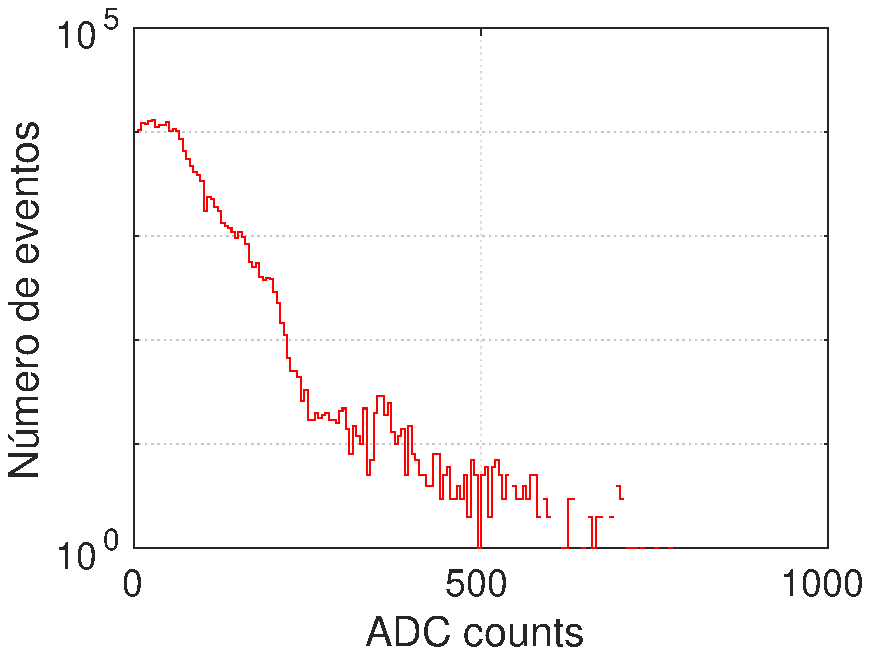
\includegraphics[width=7cm]{textuais/dadosreais/figuras/peakdist.pdf}
	\caption{Left: distribuição de picos com problema causado pela estimação. Right: Distribuição de picos após a resolução do problema de estimação}
	\label{fig:peakdist}
\end{figure}

\section{Dados da aquisição}

Após resolver os problemas de saturação e estimação dos sinais, temos os dados  a serem comparados com a simulação, representados pelas Figuras \ref{fig:peakdist} e \ref{fig:hist_evt}.
A Figura \ref{fig:peakdist} representa a distribuição de p.e. para todas as PMTs indivitualmente.
A Figura \ref{fig:hist_evt} representa a quantidade de p.e. por evento, ou seja, a soma do número de p.e. estimados por evento de todas as PMTs do detector central. 
\\

\begin{figure}[H]
	\centering
%	\hspace*{-2cm}
	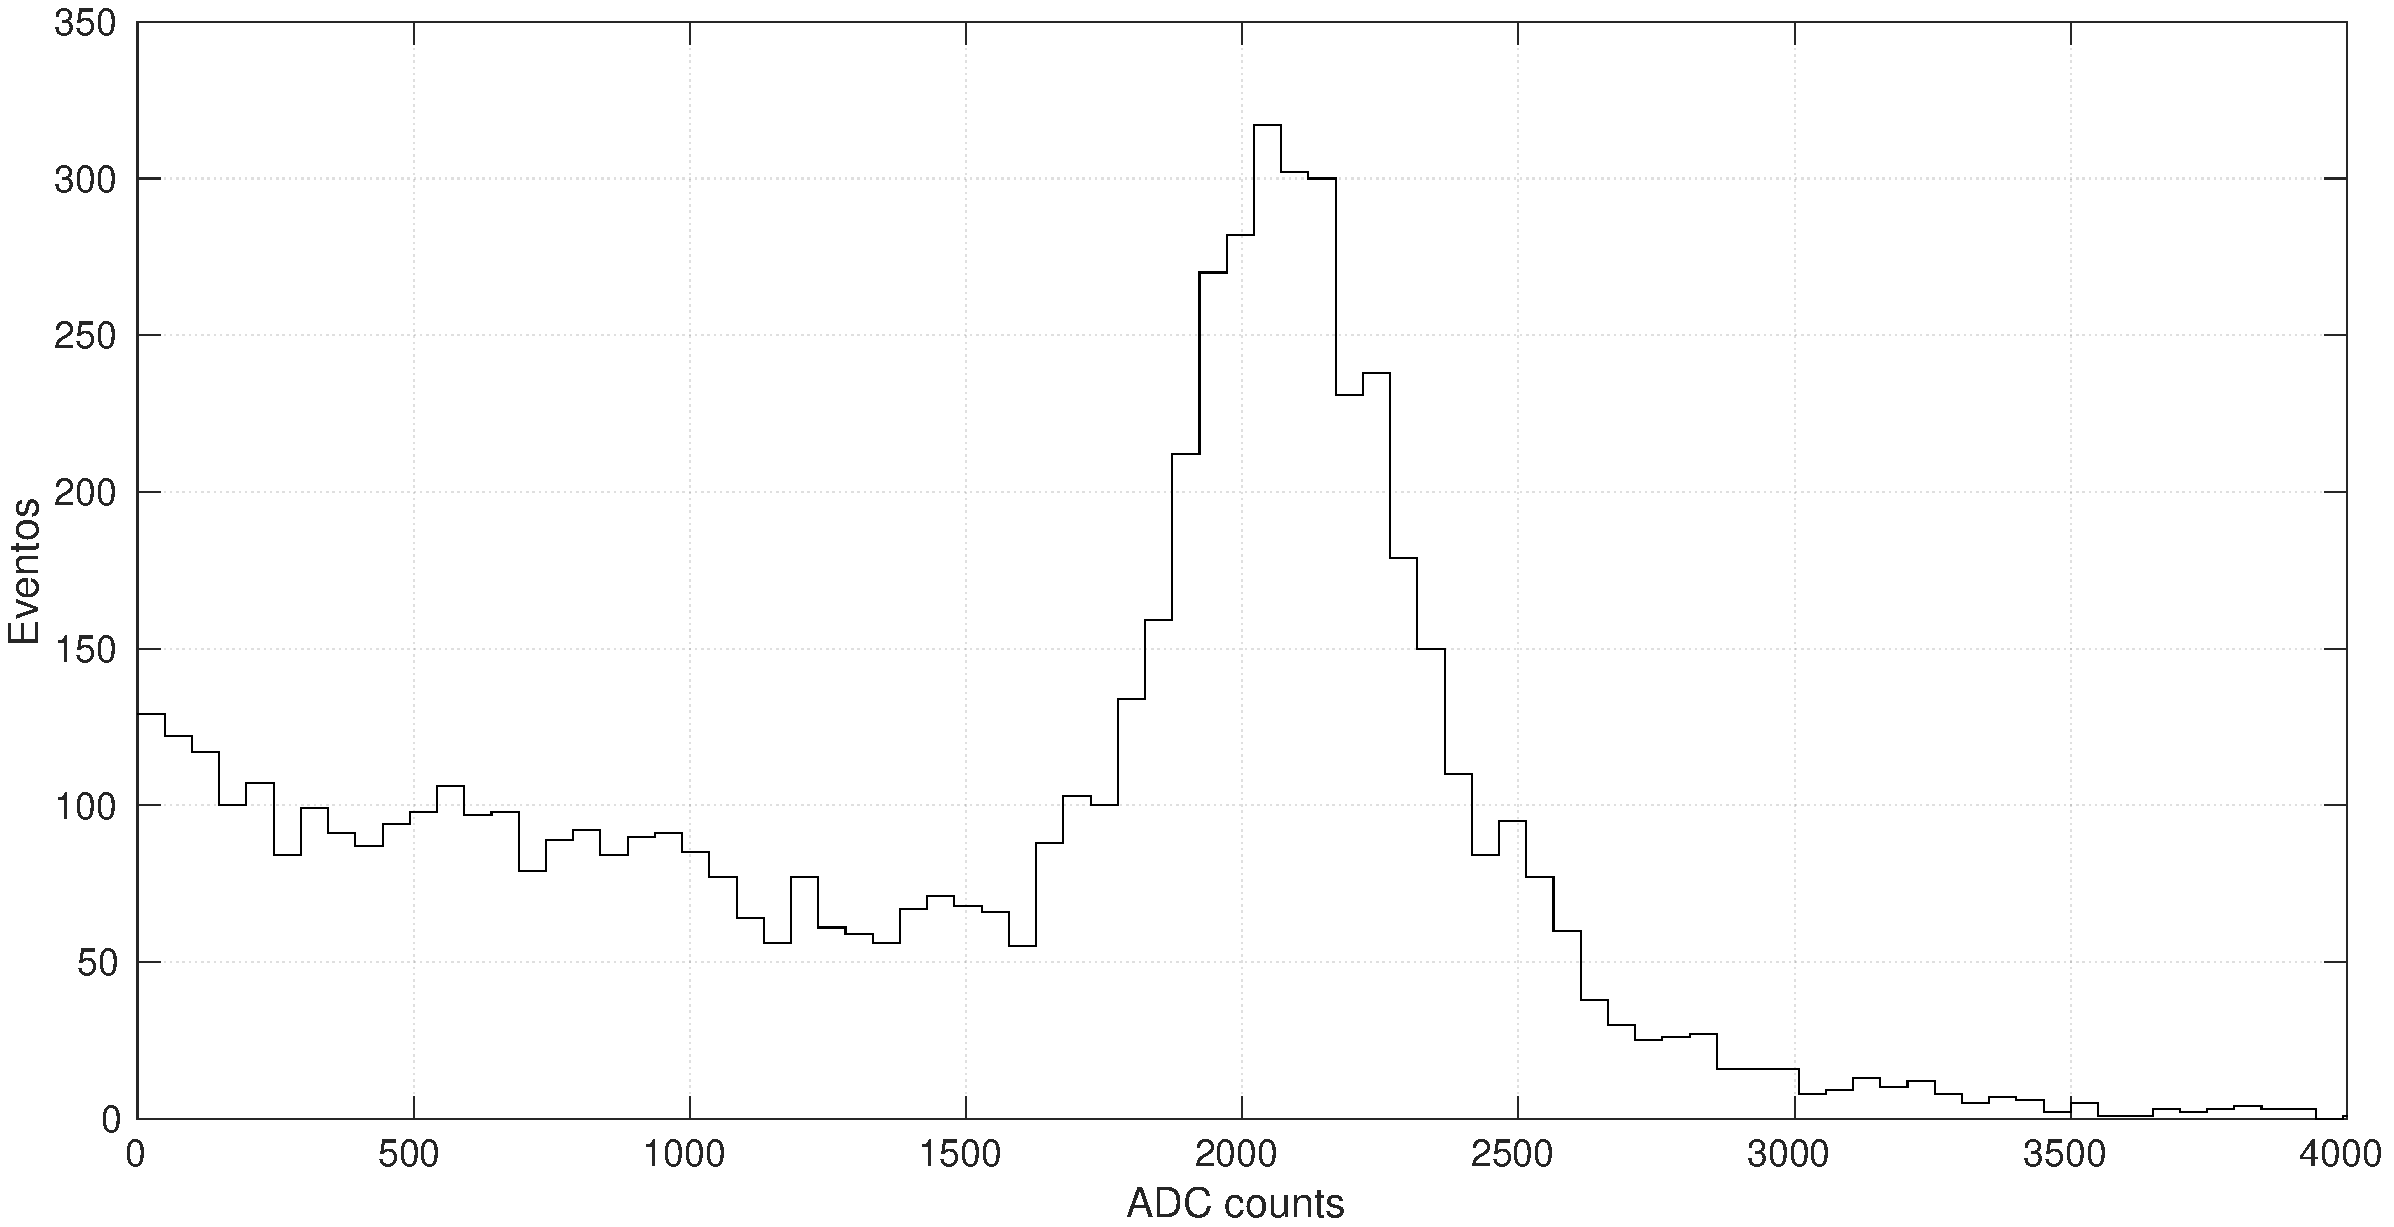
\includegraphics[width=12cm]{textuais/dadosreais/figuras/FigureName_Fig_5.pdf}
	\caption{Distribuição de picos após a resolução do problema do \emph{fit}}
	\label{fig:hist_evt}
\end{figure}

\subsection{Outros dados importantes}

Embora a análise apresentada nesse projeto esteja focada nos níveis de energia nas PMTs e nos eventos, outras análises também são importantes para este trabalho, como, por exemplo, os gráficos apresentados nas Figuras \ref{fig:probsubinf_real} e \ref{fig:firedpmt_real}.
A Figura \ref{fig:probsubinf_real} representa a probabilidade da PMT mais energética de um evento estar entre as $16$ PMTs superiores ou entre as $16$ inferiores.
A Figura \ref{fig:firedpmt_real} representa a distribuição de número de PMTs disparadas por evento.
Essas figuras são importantes para a validação da calibragem dos parâmetros da simulação no Capítulo \ref{cap:resultados}.

\begin{figure}[H]
	\centering
%	\hspace*{-2cm}
	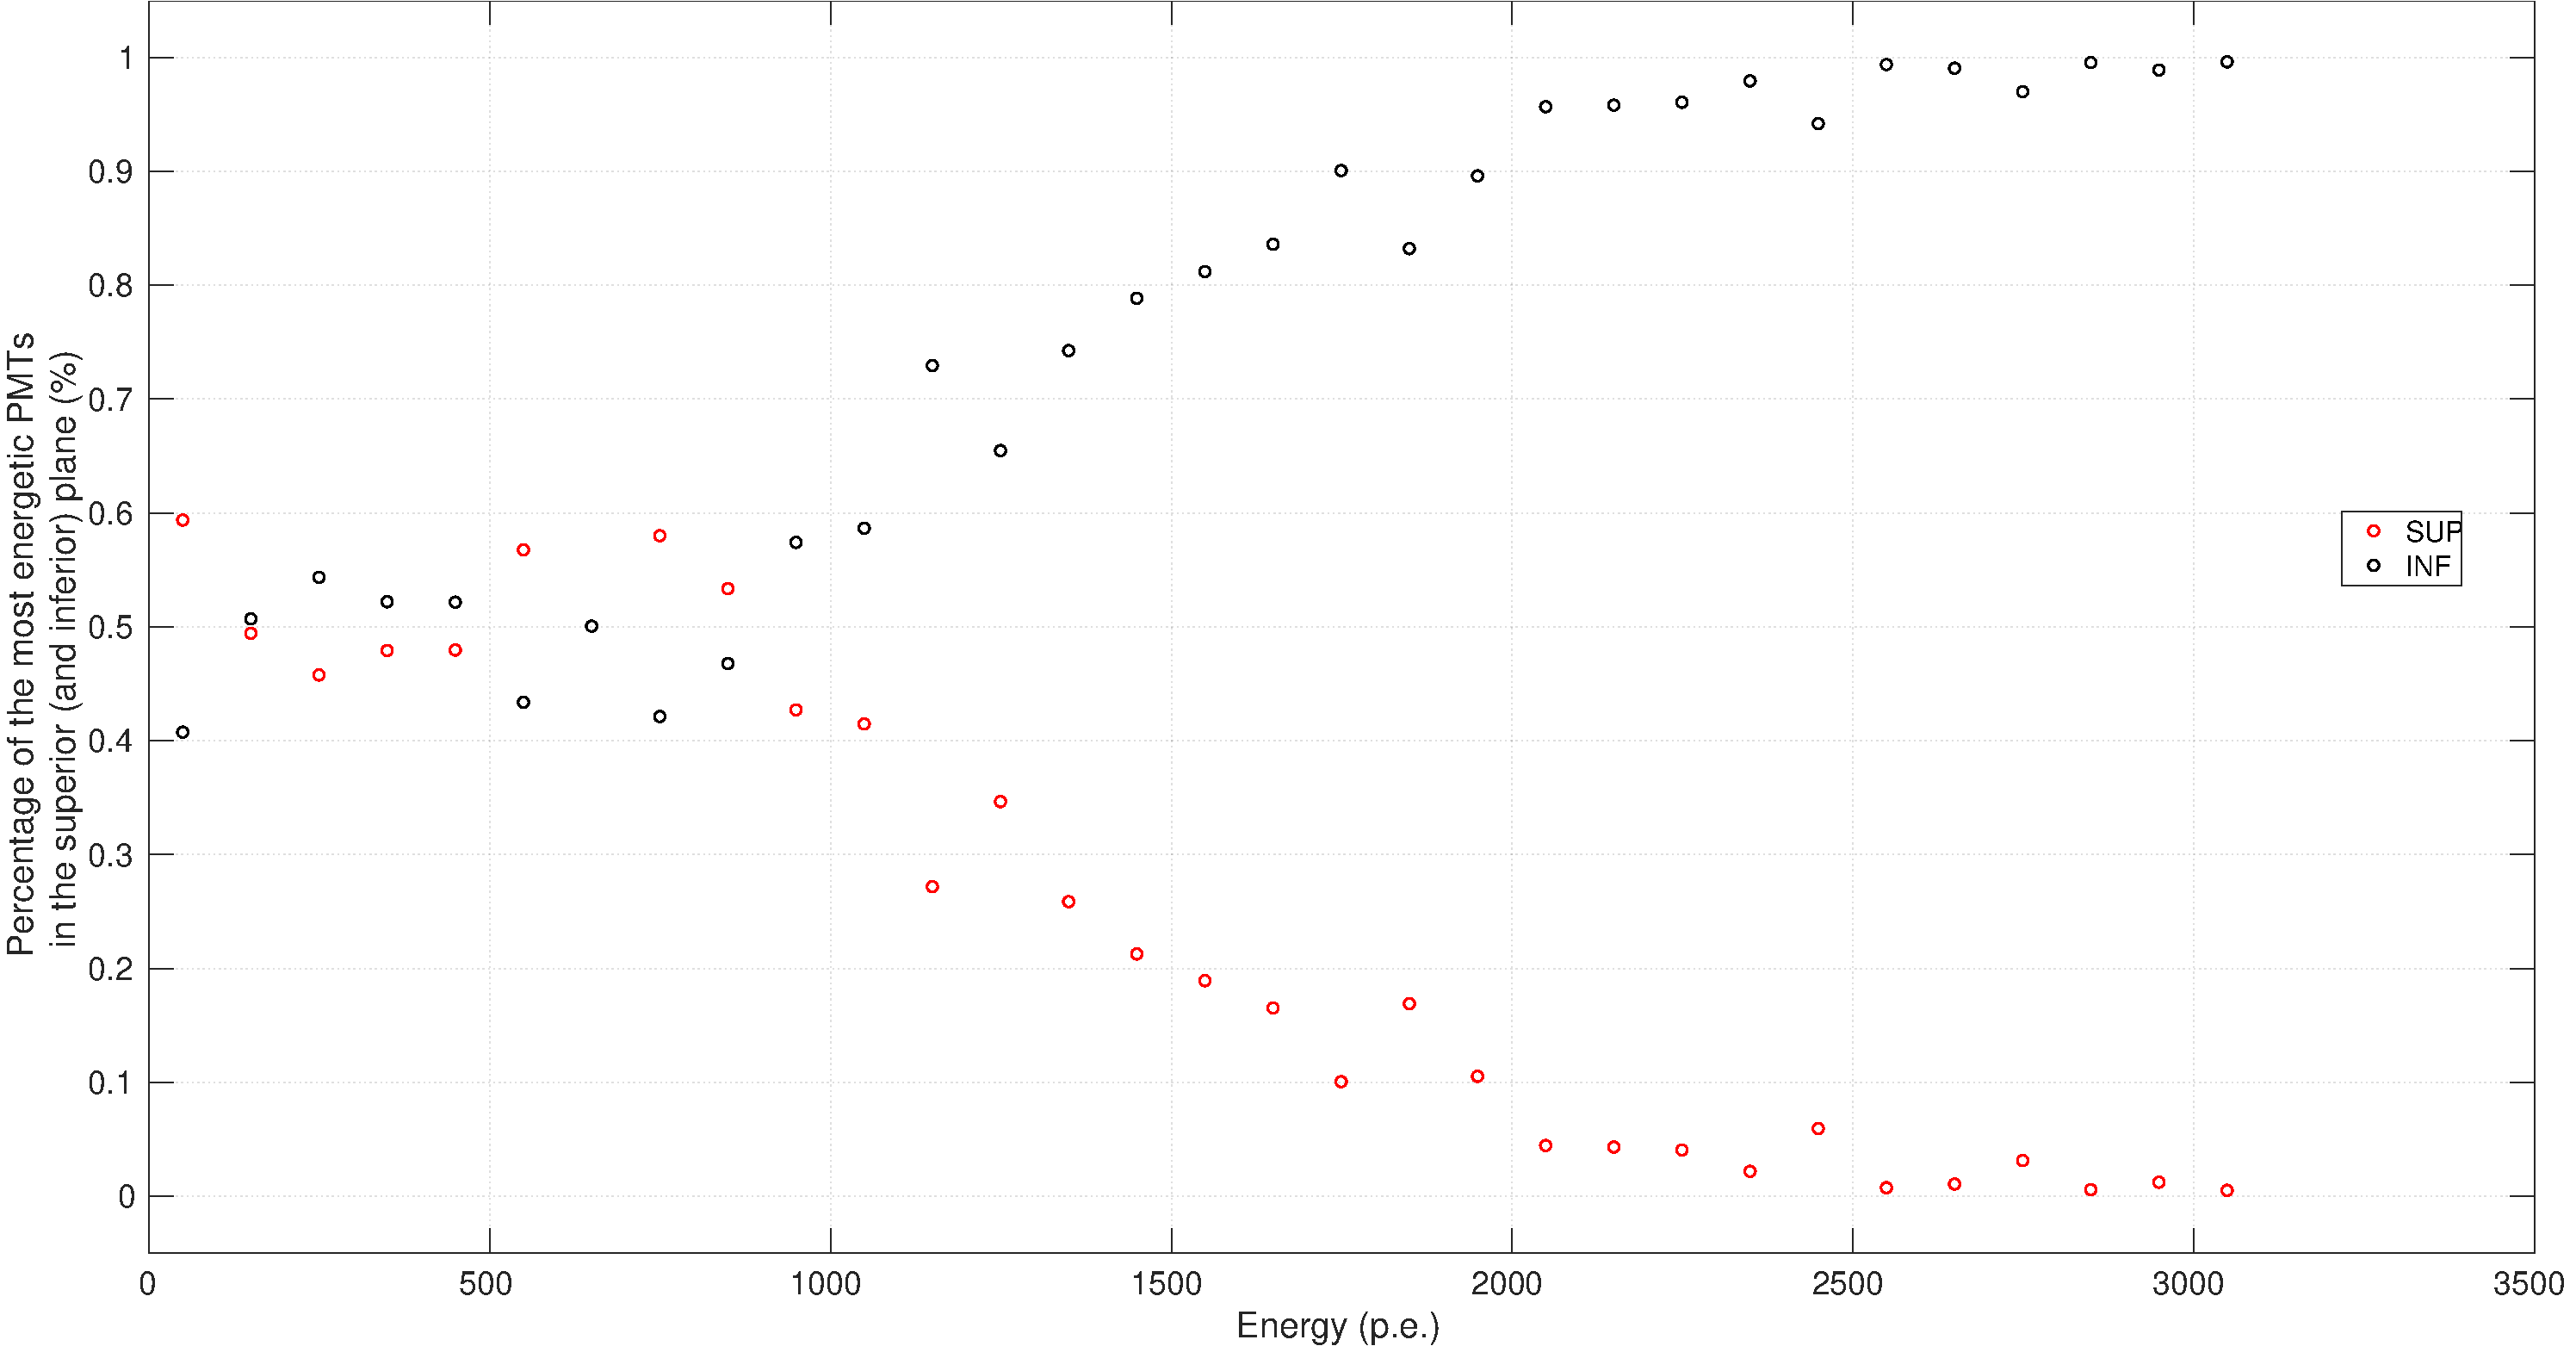
\includegraphics[width=12cm]{textuais/dadosreais/figuras/probsupinf_real.pdf}
	\caption{Probabilidade de posição da PMT mais energética}
	\label{fig:probsubinf_real}
\end{figure}


\begin{figure}[H]
	\centering
%	\hspace*{-2cm}
	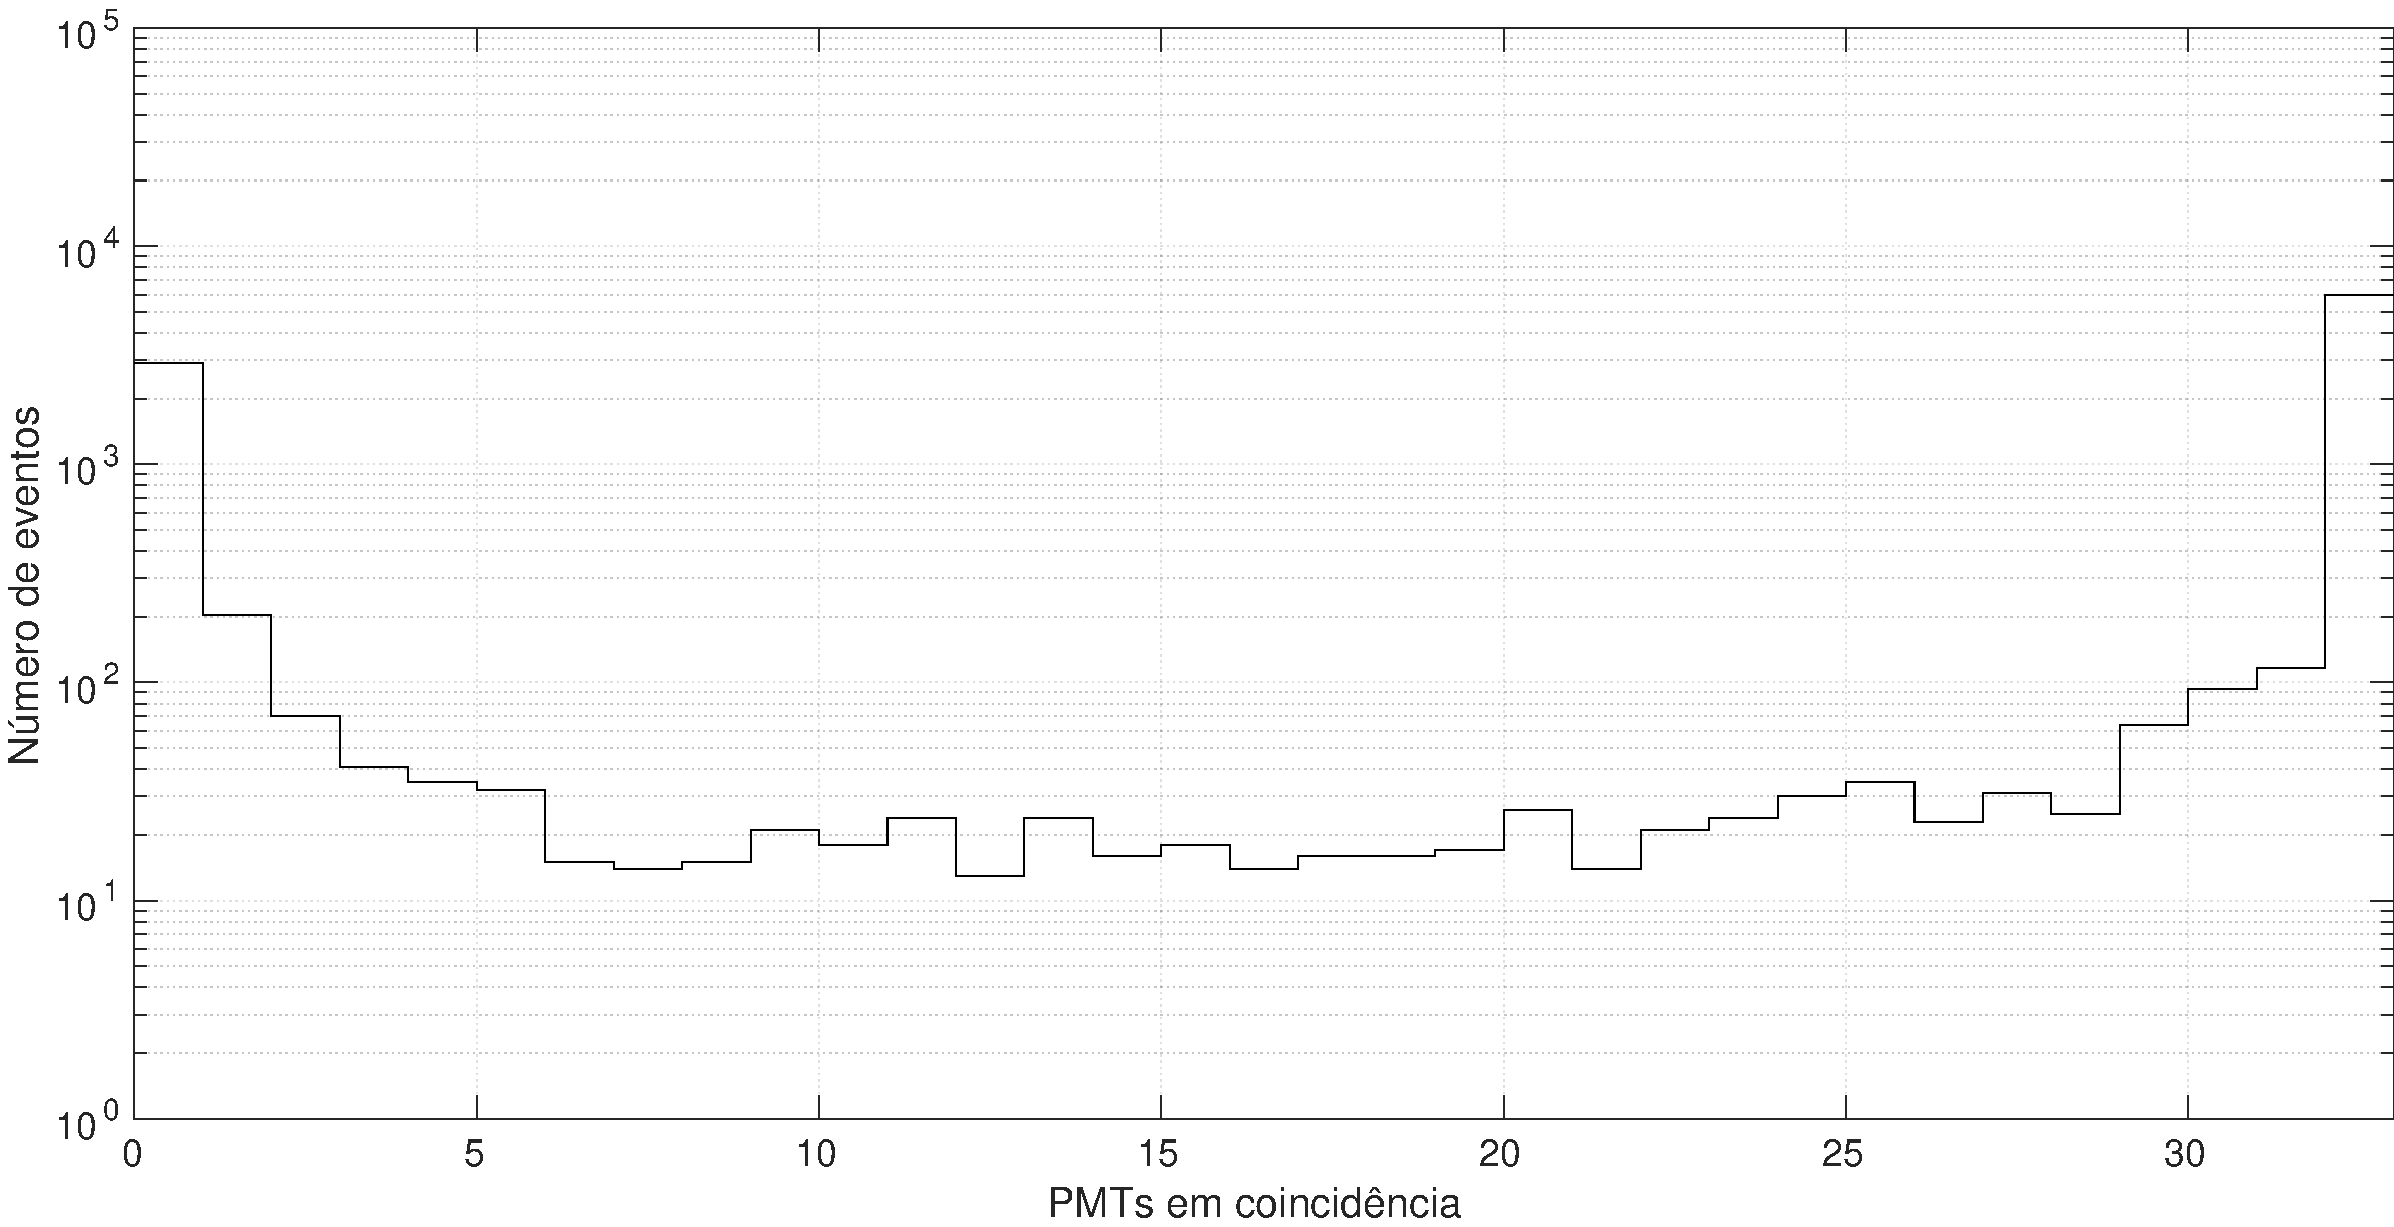
\includegraphics[width=12cm]{textuais/dadosreais/figuras/firedpmt_real.pdf}
	\caption{Distribuição de multiplicidade por evento}
	\label{fig:firedpmt_real}
\end{figure}

Outros plots podem ser encontrados no apêndice \ref{apdx:dadosreais}.